\chapter{Introduction}

% Justify & highlight the problem
Behavioral analysis and the analysis of mental health and development from videos utilizing computer vision algorithms is a relatively newer field adopted in the Autism community. Most works done till date try to interpret and identify the objects present in the scene and extract physical and geometrical parameters like pose, orientation, location, etc. Along similar lines, the gaze of a subject and the proximity of the subject’s face from the recording device are some of the important features utilized for gauging the social and non-social preferences of the subject in the Autism community and carrying out various mental health assessments.

In this direction, we prepare a Gaze Tracking dataset containing videos of children aged 0-6 years performing Preferential Looking Task on a tablet in indoor settings. This dataset is targeted toward the screening and classification of Autism Spectrum Disorder (ASD) in small children and will be helpful for the Autism community. Before releasing the dataset to the community, the primary concern is the redaction of the identities of the subjects present in the video (since our dataset is subject to GDPR regulations). So, our aim is to share a face redacted dataset while preserving the gaze and facial proximity features of the subjects. In this work, we aim to systematically demonstrate our feature preserving approach to face redaction using the ITracker neural network as the base model introduced by \cite{MIT_EyeTracking_paper} and prepare a feature-rich face redacted dataset.


%%%%%%%%%%
\section{Face Redaction}
Redaction refers to the process of hiding some sensitive information present in an image in order to preserve the privacy of individuals. The sensitive information can be present in the foreground or the background of the image. An example of the redaction of the foreground is the face redaction problem, which aims at preserving the identities of the subjects present in the videos. There are several ways in which the faces can be redacted, e.g., by blurring or blackening out all the faces, swapping the face with the face of another person, or overlaying a mesh of facial landmarks. For the sake of simplicity, we blur or blacken out the faces present in the video. The various modalities in which face redaction can be achieved are demonstrated in figure \ref{fig:faceRedactModes}. The face can either be blurred or completely blacked out to hide the identity, or the facial landmarks can be overlaid on the black background or the blurred face. As we will demonstrate the importance of eyes for gaze tracking in upcoming sections, the eyes can either be hidden or visible in each of the above modalities.

\begin{figure}[tbp]
  \centering
    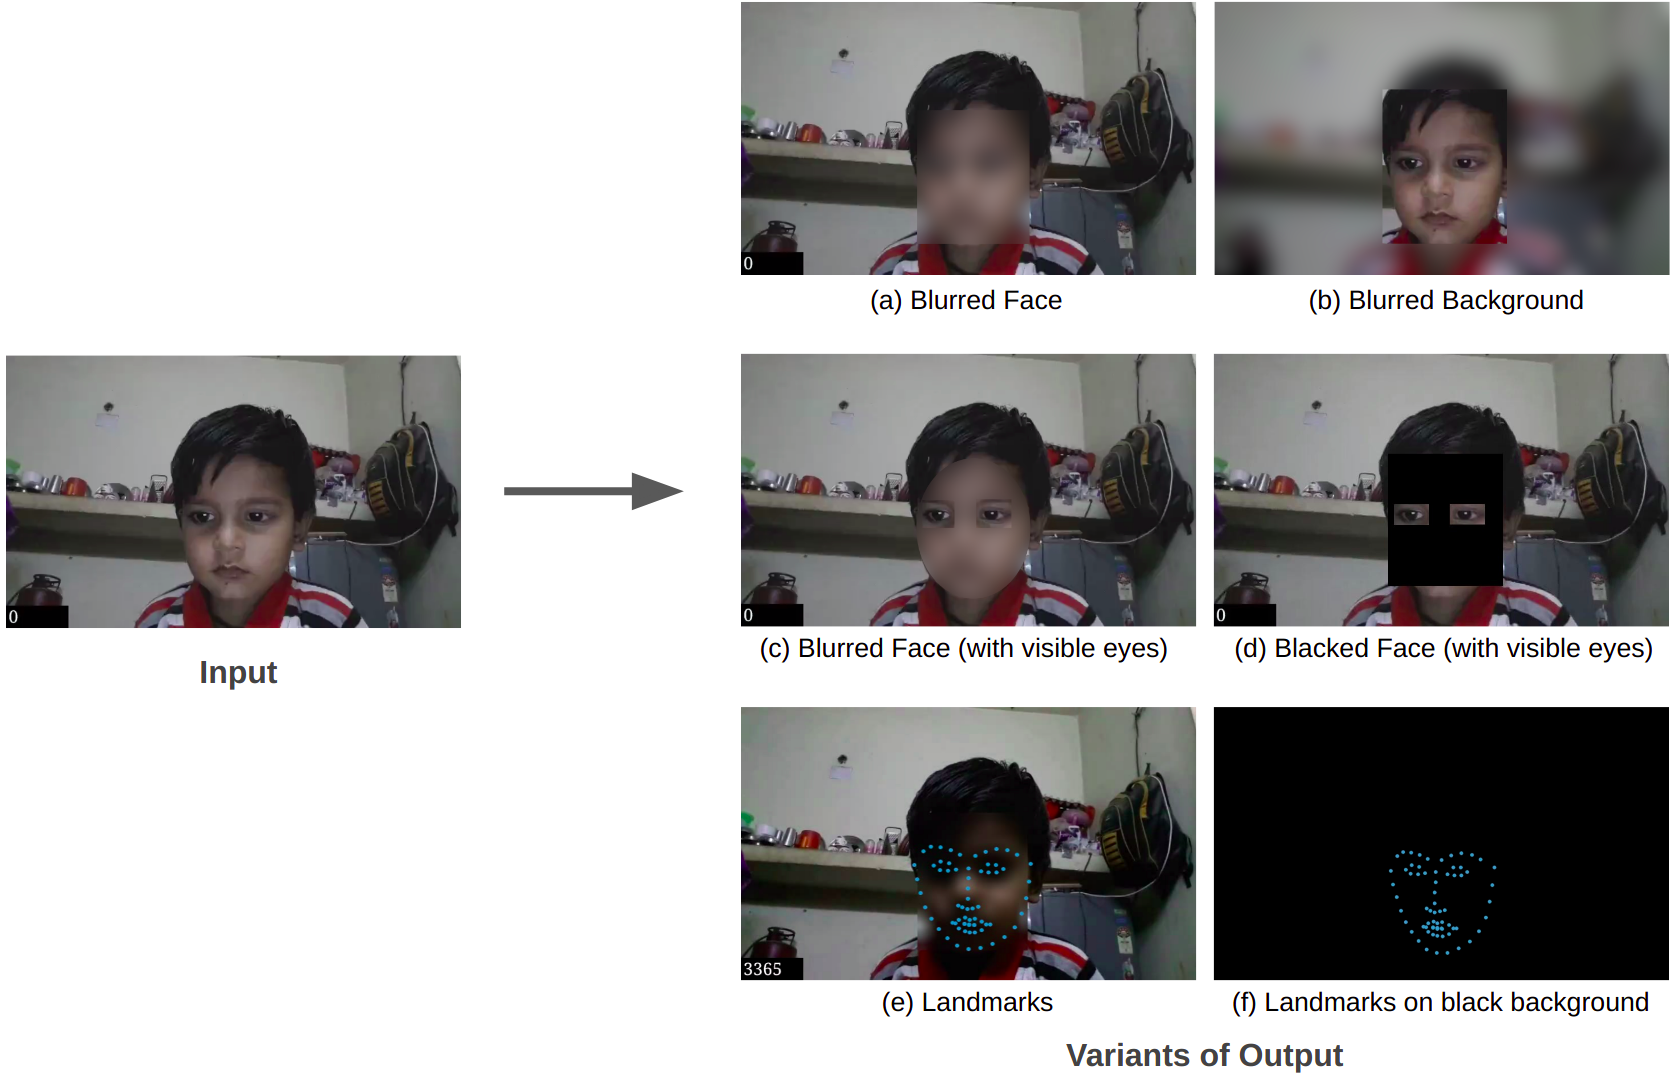
\includegraphics[width=1.0\textwidth]{Introduction/FaceRedactionModalities}
    \caption[Redaction Modalities]{Redaction modalities}
    \label{fig:faceRedactModes} 
\end{figure}

While this procedure is of utmost importance before releasing the dataset to the community, it makes it difficult to extract gaze and facial proximity features from these redacted faces. Thus, a feature preserving redaction mechanism needs to be adopted.


%%%%%%%%%%
\section{Gaze Classification}
Gaze refers to the direction in which an individual is looking and focusing at. This is an important feature of an individual's behavioral aspect which makes the tracking of an individual's gaze very vital in order to study the attention of the individual. The task of Gaze Tracking (or sometimes Eye Tracking) refers to the use of an external device to follow an individual’s gaze and eye movement, which is used for various studies, including studies of the visual system, cognition, and psychology. In such applications, one is typically interested in the classification of gaze into Left or Right regions (called 2-Way Classification, figure \ref{fig:2wayGazeClassif}) or Left, Right, or Middle regions (called 3-Way Classification, figure \ref{fig:3wayGazeClassif}) of the device on which the eye-tracking data is collected. An application running on a device (say, a mobile phone) displays a dot (fixation point), the subject looks at the fixation point, video of the subject is recorded using the front camera of the device, which is used to monitor the screen location where the subject is looking at.\\

\begin{figure}[h]
    \centering
    \captionsetup[subfigure]{justification=centering}
    \subfloat[2-Way Gaze Classification on Preferential Looking Task]{{
        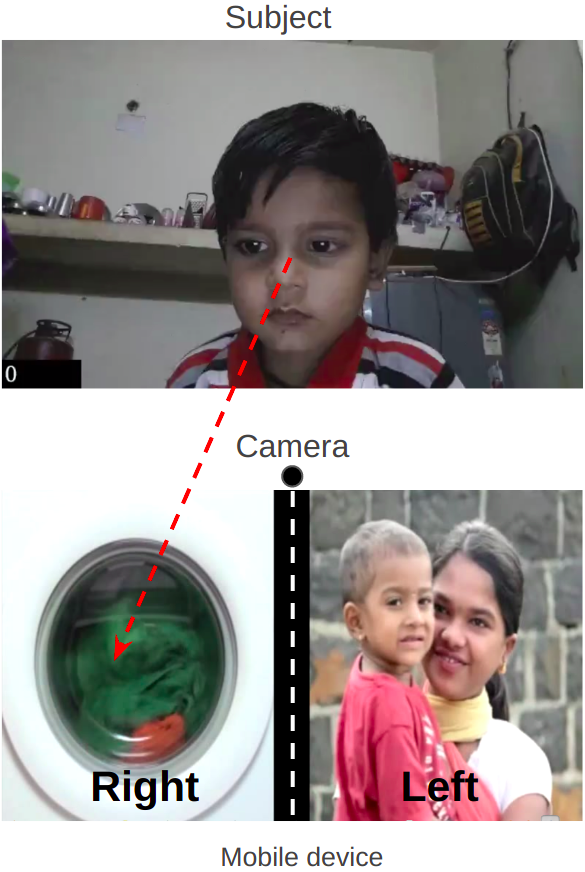
\includegraphics[scale=0.3]{Introduction/2wayGazeClassif}
        \label{fig:2wayGazeClassif}
        }}
    \qquad
    \subfloat[3-Way Gaze Classification on Anti-Saccade Task]{{
        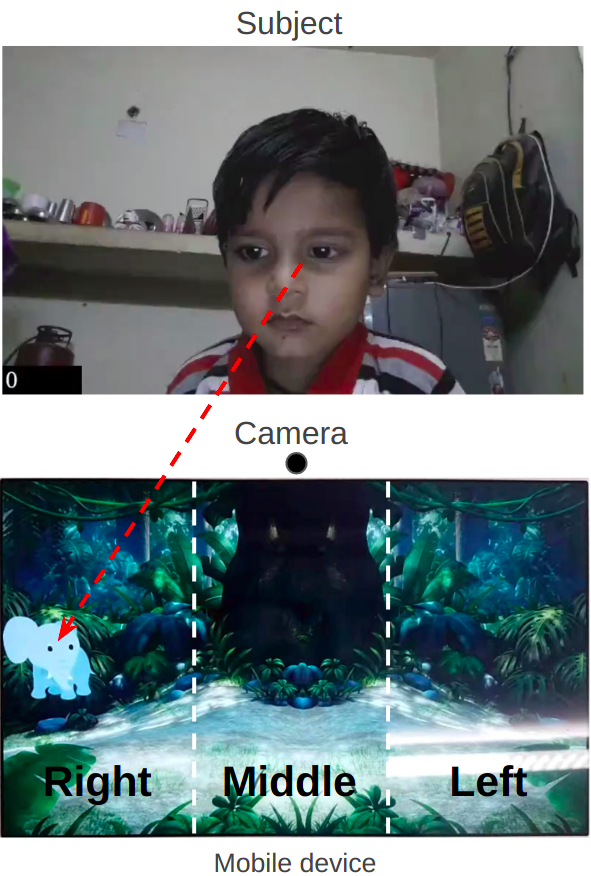
\includegraphics[scale=0.3]{Introduction/3wayGazeClassif}
        \label{fig:3wayGazeClassif}
    }}
    \caption{Gaze Classification}
\end{figure}


%%%%%%%%%%
\section{Facial Proximity}
The proximity of the face to the camera of the recording device is an important feature for gauging the attention of the subject. We extract the 3-D facial landmarks using the state-of-the-art facial landmark detector, RetinaFace \citep{retinaFace2020} and calculate the relative 3-D proximity of the nose-tip from the camera across consecutive frames of the video.

\begin{figure}[h]
  \centering
    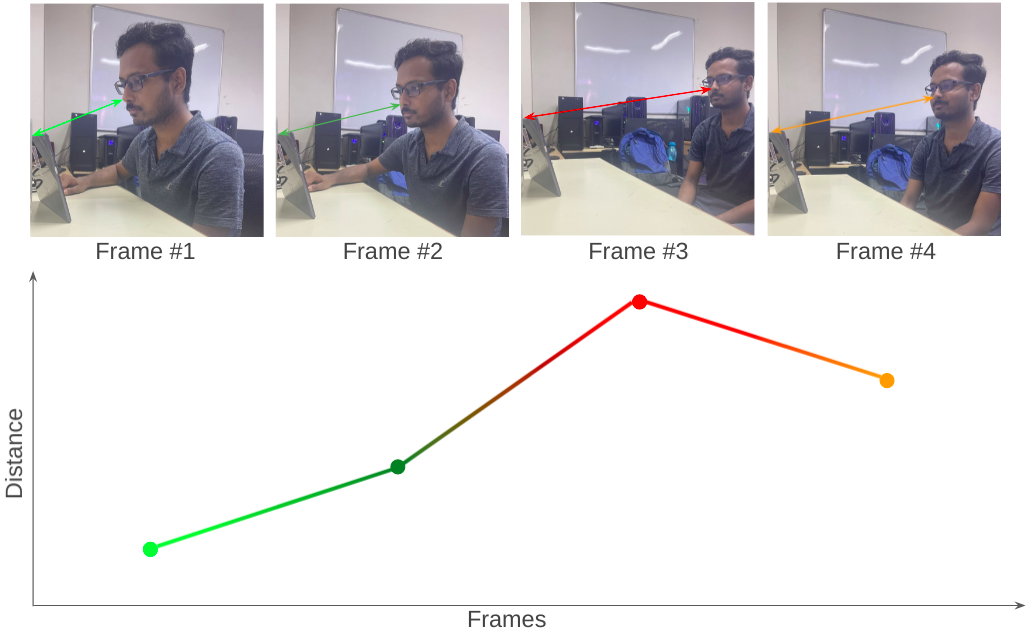
\includegraphics[width=0.85\textwidth]{Introduction/RelFaceDist}
    \caption[Relative Face Proximity]{Relative 3-D proximity of nose-tip from camera across consecutive frames}
    \label{fig:relFaceDist} 
\end{figure}


%%%%%%%%%%
\section{Motivation and Applications}
We need to share our prior work and results obtained on our Gaze Tracking dataset. Given that our Gaze Tracking Dataset is subject to GDPR regulations, identity preservation is imperative, without which we can’t share the dataset. Therefore, we aim to prepare and share a redacted dataset with eye crops and facial landmark coordinates in order to establish the utility of our redacted dataset for gaze classification and facial proximity calculation. With redacted faces and eye crops present in our dataset, we can calculate the gaze of an individual. The landmarks supplied along with our dataset can be used to compute the facial proximity of individuals. Our dataset can also be used for the exploration of new algorithms on a redacted dataset for research purposes.

This work finds applications in many domains. For example, gaze tracking in remote exam settings is important for tracking whether the student is looking at the screen. Malpractice detection without revealing a student’s identity in such remote exam settings is very helpful for academia. Another important metric is face distance and proximity, which is very helpful in gauging the attention of an individual. Such a pipeline can be incorporated into software applications such as SafeEyes (a Linux-based software for the protection of eyes from excessive screen exposure) without breaching the privacy of the user.

\section{Contributions}
As discussed in previous sections, the task of face redaction makes the image lose the important facial features which are required for gaze classification and proximity calculation. We propose a feature preserving face redaction pipeline, which is useful for sharing a privacy preserved dataset to the research community. Furthermore, we demonstrate the utility of such a face redacted dataset by performing several experiments and ablation studies for gaze classification on this dataset. We show that our approach to gaze classification works equally well on face redacted data as it performs on the unredacted data. Specifically, we achieve a 3-way gaze classification accuracy of 82\% and a 2-way gaze classification accuracy of 96\% on UK dataset. We test our approach on the uncurated START data collected using Preferential Looking task and achieve a 2-way classification accuracy of 93\% with redacted faces. We also proposed an algorithm to calculate the proximity of the face of an individual from the camera and demonstrate the proximity trends on various in-the-wild videos. We plan to make the trained models and face redacted dataset (along with the facial features in terms of facial landmarks and eye crops) available to the research community for further investigations and research work.